\chapter{VRPTW via Optimization}
In this chapter, we review, multiple approaches for solving \gls{vrptw} via optimization techniques with the objective to find suboptimal solutions in a reasonable time. The real-life use cases of \gls{vrp} are demanding to quickly find a good enough solution for large instances and this is achieved by applying handcrafted heuristics.

\begin{figure}[ht]
    \centering
    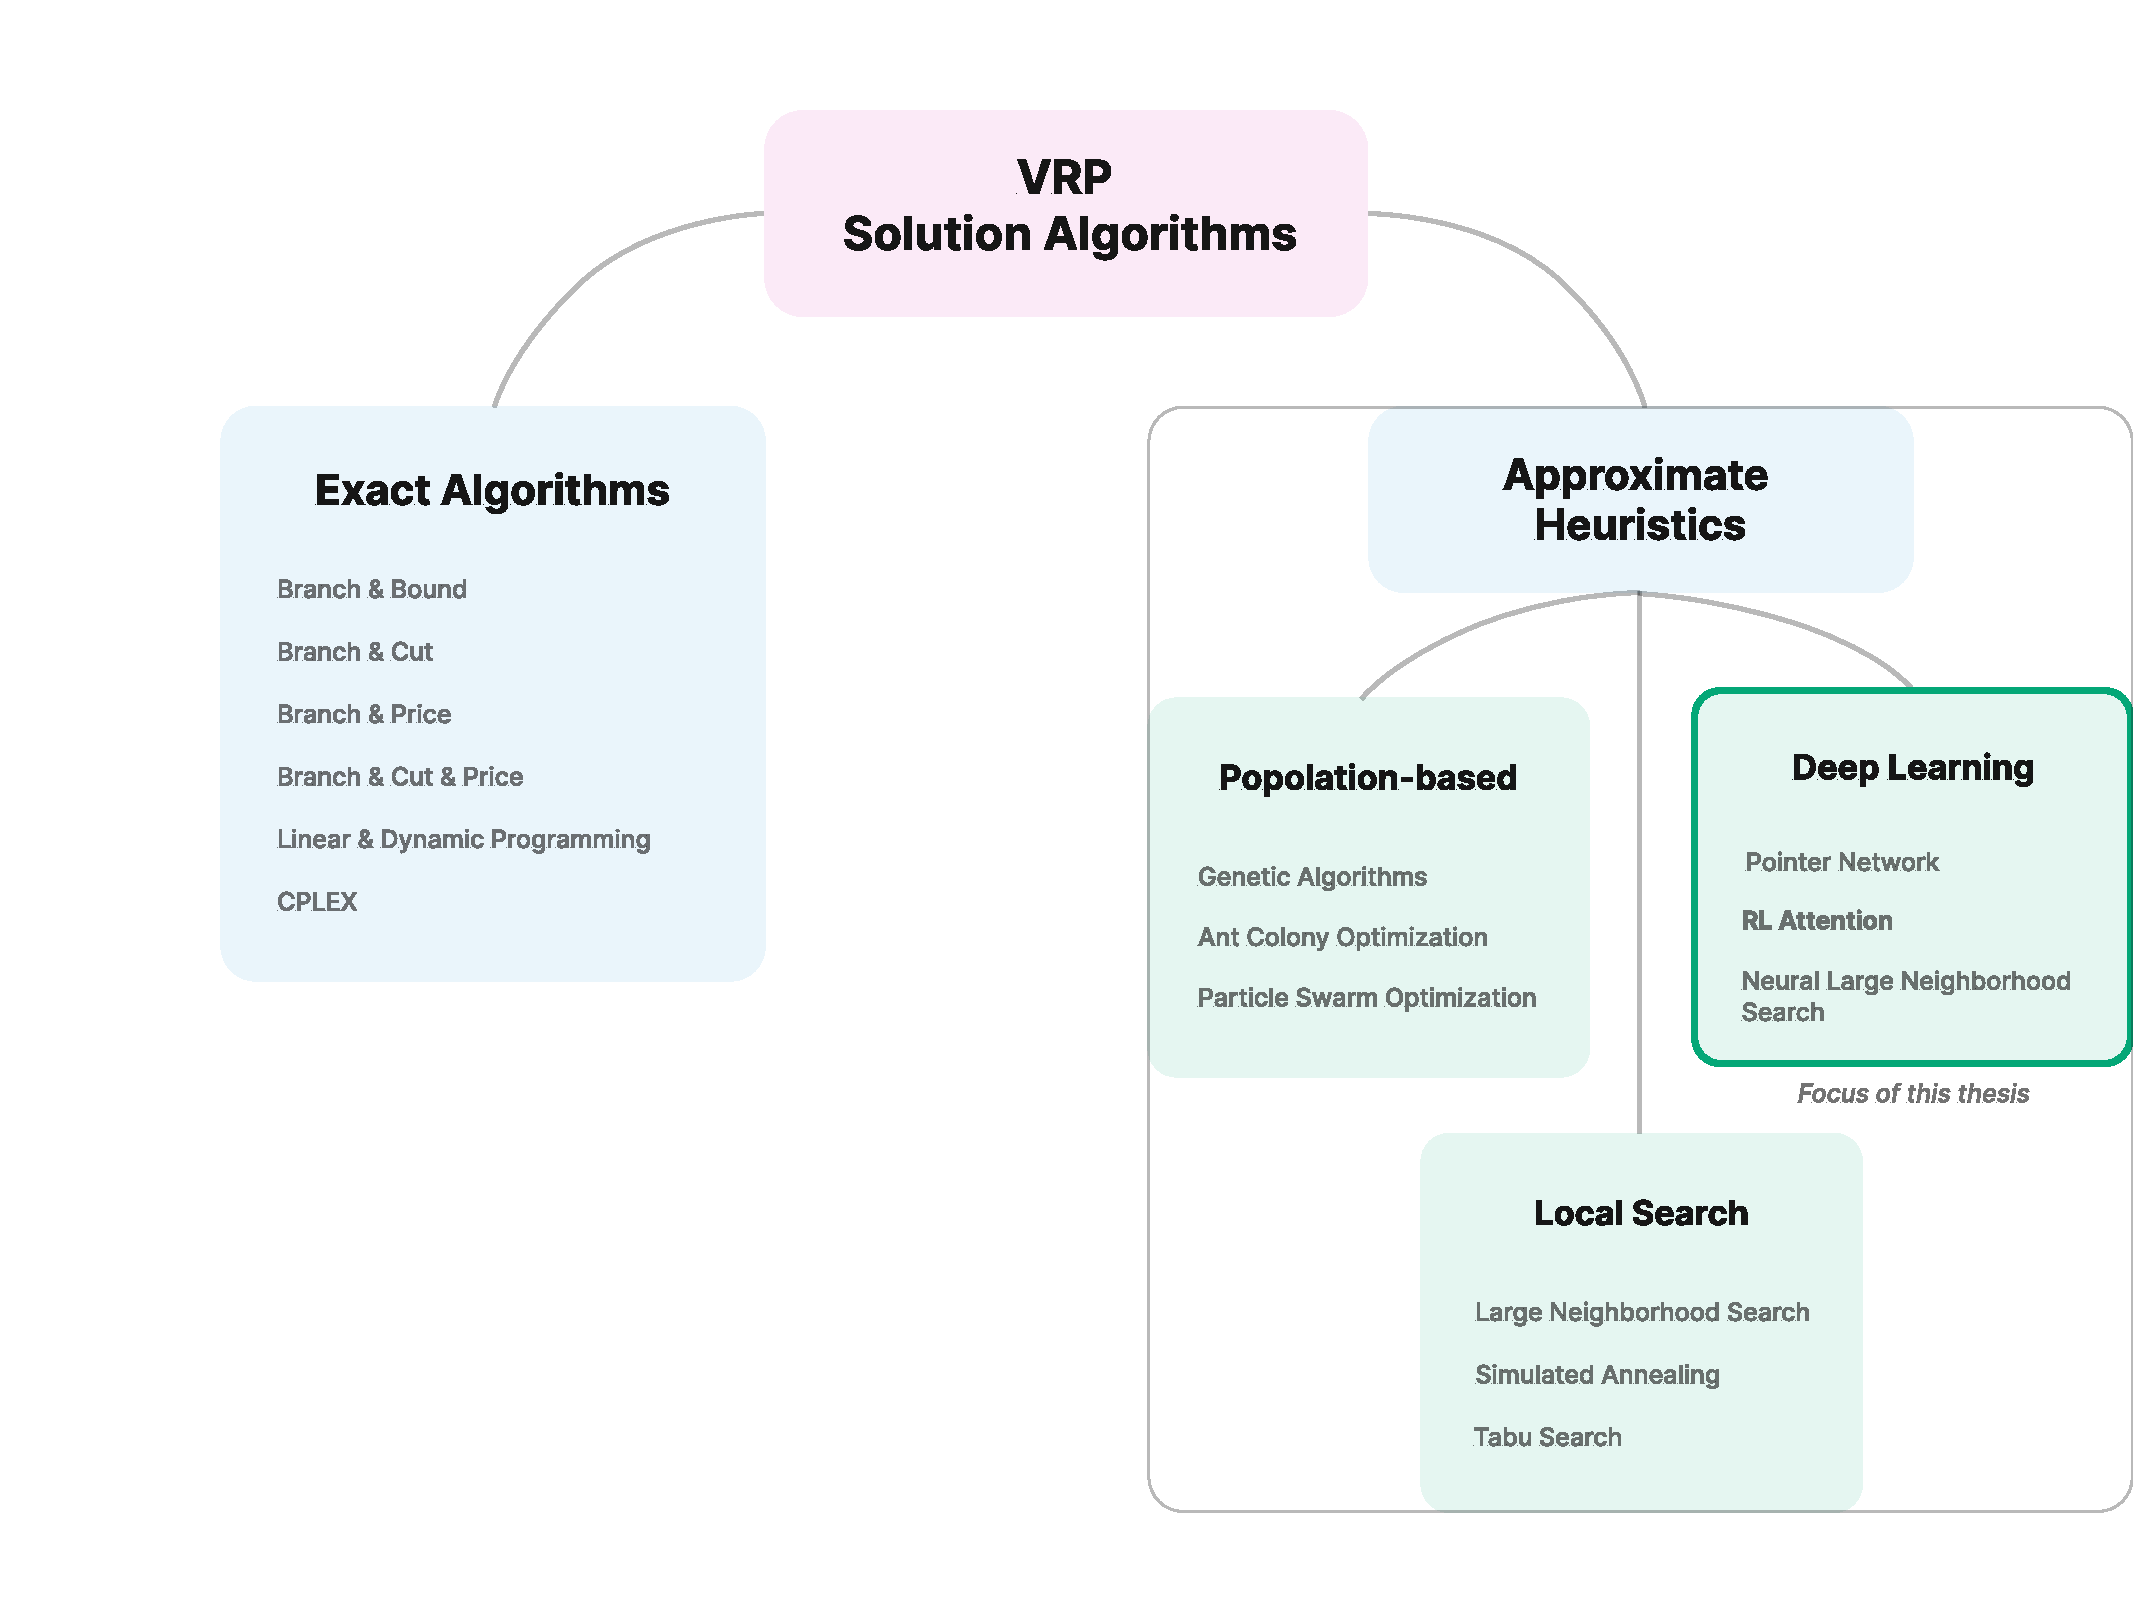
\includegraphics[width=1.0\textwidth]{resources/vrptw-optimization/vrp-solutions.pdf}
    \caption{Family of algorithms for solving \gls{vrp}}
    \label{fig:vrp-graph}
\end{figure}

In the field of operations research, approximate heuristics may be divided into \emph{constructive heuristics} and \emph{metaheuristics}. Constructive heuristics are used to provide an initial solution in a matter of seconds, which is later optimized. Metaheuristics is end-to-end algorithm that takes a problem instance and calculates its suboptimal solution. Metaheuristics can be further divided into \emph{local search method} which explores the search space by iterativly moving to a better solution, or \emph{population-based methods} that generate a set of solutions that are continually evolving \cite{vrp-bible}.

\section{Insertion Heuristics}
Insertion heuristic is a constructive heuristic first proposed by Jang-Jei Jaw et. al \cite{i1-heuristics} in 1986.
        
\section{Google OR-Tools}
We have noticed that many of the production solutions in the field of logistics use some type of optimization framework. The framework allows to describe the routing problem using their specific notation and their optimization library finds its solution. They usually implement variants of local search algorithms. However, their are fairly flexible and they serve as a great reference point for any benchmarking.

In this thesis, we use Google OR-Tools\footnote{\url{https://developers.google.com/optimization}} an open source tool developed to solve optimization problems in vehicle routing, network flows, integer and linear programming, and constraint programming \cite{ortools}. We have chosen this optimization framework because the operations research community uses OR-Tools as a main benchmark and it supports soft constraint programming.

OR-Tools works by building a graph where the distance callback function assigns a value to graph transitions called arc cost. In the use case of solving \gls{vrptw}, the arc cost is supposed to be the traveled duration between two given locations (nodes). 

OR-Tools implements a cost function in the form of dimensions representing quantities accumulated at nodes along the vehicle's route. Solving \gls{vrptw} via OR-Tools requires to have extra dimensions for time windows that accumulates early and late arrivals. OR-Tools are minimizing the dimensions values by using a chosen metaheuristic. 

OR-Tools implements many well-known metaheuristics such as
\begin{itemize}
        \item AUTOMATIC Lets the solver select the best metaheuristics.
        \item GREEDY\_DESCENT Accepts only cost-reducing solutions using local search of neighbors until a local minimum is reached.
        \item GUIDED\_LOCAL\_SEARCH Uses guided local search to escape local minima \cite{guided-local-search}.
        \item SIMULATED\_ANNEALING Uses simulated annealing to escape local minima \cite{simulated-annealing}.
        \item TABU\_SEARCH Uses tabu search to escape local minima \cite{tabu-search}.
        \item OBJECTIVE\_TABU\_SEARCH Uses tabu search on the objective value of a solution to escape local minima \cite{objective-tabu-search}.
\end{itemize}

\section{Large Neighborhood Search}\ref{lns}
Heuristics based on large neighborhood search have shown superior results in solving a wide variety of routing problems. Large neighborhood search was first introduced by Shaw \cite{shaw-lns} in 1997.

Large neighborhood search is an iterative algorithm that gradually improves its solution by exploring its neighborhoods. The neighborhoods are defined by applying \emph{destroy} and \emph{repair} operator. The destroy operator removes a random part of the solution such that different parts are destroyed in each iteration. The repair operator takes the partial solution and rebuilds into a fully feasible solution \cite{lns}.

In the implementing of large neighborhood search, the most important is to pick the proper degree of destruction for the destroy operator. If it destroys a small part of the solution, then it leads to ineffective exploration of the search space. In the opposite, when destroying large parts of the solution, the algorithm will keep re-optimizaing, which yields poor quality solutions with higher complexity \cite{lns}. The degree of destruction can be either chosen randomly or it can be gradually increased during the execution.\newline

\begin{algorithm}[H]
    \SetAlgoLined
    Initialize a feasible solution $x_b$;
    
        \While{stopping criteria is met}{
    
            $x_t$ = repair(destroy($x_b$));
            
            \If{accept($x_t$, $x$))}{
                Accept a new solution $x = x_t$;
            }
            
            \If{cost($x_t$) $>$ cost($x_b$)}{
                
                Keep the best $x_b = x_t$;
            
            }
        }
        return $x_b$;
    \caption{Large Neighborhood Search}
\end{algorithm}

The original large neighborhood search algorithm only accepted a superior solution based on the cost function. To achieve better exploration, a new acceptance criterium was used, inspired by the algorithm of simulated annealing \cite{lns-anneling}. The algorithm accepts the solution $x$ based on probability $e^{(c(x_t) - c(x))/T}$ where $T$ is the parameter for temperature. The temperature is gradually decreasing resulting in accepting fewer deteriorating solutions.

\subsection{Adaptive Large Neighborhood Search}
Adaptive Large Neighborhood Search is an extension of \gls{lns} that was proposed by Ropke et. al \cite{alns} in 2006.

\gls{alns} supports multiple destroy operators and repair methods and adds a component of diversification strategy.

% and insertion operators are selected based on their past performance during the search, usually by employing a roulette wheel selection process with an adaptive weight adjusting mechanism \cite{Azi2014, Gschwind2016, Masmoudi2020}. Ropke and Pisinger (2006) \cite{Ropke2006} used the adaptive large neighborhood search heuristic to solve the PDP with time windows. Their algorithm used removal and insertion operators already existing in the literature, including the removal operator by Shaw (1997) \cite{Shaw1997}, and an acceptance criterion for new solutions known from simulated annealing. The algorithm by Ropke and Pisinger has proven to be powerful and has served as a building block for many further studies in complicated routing problems, particularly PDP and DARP \cite{Gschwind2016, Braekers2016, Masmoudi2016, Belhaiza2017, Drexl2018, Belhaiza2019, Masmoudi2020, Wang2020, Cauchi2020, Malheiros2021}. Gschwind and Drexl (2016) \cite{Gschwind2016} adopted the algorithm from Ropke and Pisinger and added three more removal operators. They also demonstrated how to test a new solution for feasibility in an amortized constant time. Their version of the adaptive large neighborhood search produced better solutions on standard DARP instances compared to the vast majority of other algorithms, except for the hybrid genetic algorithm by Masmoudi et al. (2017) \cite{Masmoudi2017}.
% \vspace{0.5cm}

\section{Ant Colony Optimization}
The other category of metaheuristics are population-based methods, which take their inspiration from natural concepts such as the evolution of species or the behavior of insects. However, all successful population-based heuristics rely on local search methods to drive the search towards promising areas and to avoid local optima. As a result, the majority of population-based algorithms are naturally hybrid \cite{vrp-bible}.

Ant colony optimization was first applied on \gls{vrp} by Reimann et. al \cite{aco} in 2004, and successfully outperformed many existing solutions. It is inspired by the pheromone mechanism used by ants for coordination. where each ant simulates a solution by traversing the graph along its edges and accumulates the pheromones.

Ant Colony Optimization mainly consists of the iteration of four steps \cite{aco}: 
\begin{itemize}
        \item Generation of solutions according pheromone information.
        \item Application of a local search to the ant's solution.
        \item Update of the pheromone information.
        \item Augmentation of the attractiveness list.
\end{itemize}

The algorithm generates solutions according to pheromone information, which represents how good is the combination of two nodes. The solution is generated by running a decision step for the ants in which they decide where to move based on the pheromone information. Each ant generates $k$ feasible moves and one is picked based on the attractiveness probability \cite{aco}, evaporating pheromone. The construction process is stopped when no more feasible combinations are possible. After the ants have constructed their solutions, it is improved by applying a local search algorithm like \gls{lns} \ref{lns}. Than the pheromone trails are updated based on the achieved local optimum \cite{aso-rank} and a new attractiveness values are created based on pheromone information.
